\documentclass[supercite]{Experimental_Report}
\title{外~國~文~學~經~典~與~世~界~地~圖}
\author{阮云轩}
%\coauthor{张三、李四}
\school{计算机科学与技术学院}
\classnum{CS2404}
\stunum{U202490035}
%\costunum{U202115631、U202115631}
\instructor{谭杉杉} % 该系列实验报告模板由华科大计院教师陈加忠制作
\date{2024年11月22日}

\usepackage{algorithm, multirow}
\usepackage{algpseudocode}
\usepackage{amsmath}
\usepackage{amsthm}
\usepackage{framed}
\usepackage{mathtools}
\usepackage{subcaption}
\usepackage{xltxtra} %提供了针对XeTeX的改进并且加入了XeTeX的LOGO, 自动调用xunicode宏包(提供Unicode字符宏)
\usepackage{bm}
\usepackage{tikz}
\usepackage{tikzscale}
\usepackage{pgfplots}
%\usepackage{enumerate}

\pgfplotsset{compat=1.16}

\newcommand{\cfig}[3]{
	\begin{figure}[htb]
		\centering
		\includegraphics[width=#2\textwidth]{images/#1.tikz}
		\caption{#3}
		\label{fig:#1}
	\end{figure}
}

\newcommand{\sfig}[3]{
	\begin{subfigure}[b]{#2\textwidth}
		\includegraphics[width=\textwidth]{images/#1.tikz}
		\caption{#3}
		\label{fig:#1}
	\end{subfigure}
}

\newcommand{\xfig}[3]{
	\begin{figure}[htb]
		\centering
		#3
		\caption{#2}
		\label{fig:#1}
	\end{figure}
}

\newcommand{\rfig}[1]{\autoref{fig:#1}}
\newcommand{\ralg}[1]{\autoref{alg:#1}}
\newcommand{\rthm}[1]{\autoref{thm:#1}}
\newcommand{\rlem}[1]{\autoref{lem:#1}}
\newcommand{\reqn}[1]{\autoref{eqn:#1}}
\newcommand{\rtbl}[1]{\autoref{tbl:#1}}

\algnewcommand\Null{\textsc{null }}
\algnewcommand\algorithmicinput{\textbf{Input:}}
\algnewcommand\Input{\item[\algorithmicinput]}
\algnewcommand\algorithmicoutput{\textbf{Output:}}
\algnewcommand\Output{\item[\algorithmicoutput]}
\algnewcommand\algorithmicbreak{\textbf{break}}
\algnewcommand\Break{\algorithmicbreak}
\algnewcommand\algorithmiccontinue{\textbf{continue}}
\algnewcommand\Continue{\algorithmiccontinue}
\algnewcommand{\LeftCom}[1]{\State $\triangleright$ #1}

\newtheorem{thm}{定理}[section]
\newtheorem{lem}{引理}[section]

\colorlet{shadecolor}{black!15}

\theoremstyle{definition}
\newtheorem{alg}{算法}[section]

\def\thmautorefname~#1\null{定理~#1~\null}
\def\lemautorefname~#1\null{引理~#1~\null}
\def\algautorefname~#1\null{算法~#1~\null}

\begin{document}
	
	\maketitle
	
	\clearpage
	
	\pagenumbering{Roman}
	
	\tableofcontents[level=2]
	
	\clearpage
	
	\pagenumbering{arabic}
	
	\section{前言}

因为这是对于读物理解吸收的输入与输出，过程中难免会向个人的客观见解倾斜，加入了自我的思想与启发。故有不少地方都只是我的见解，把作品理解成我所认可的形式，还请注意甄别，望海涵。
\\探讨三观上的不同看法，常常会涉及到是非绝对的问题，本次的读物亦是如此，所以也提出点问题可以思考一下。\\
1.一个人坚信自己拥有自由意志，可他的每一个决定都受到其成长环境、社会文化、个人经历等诸多因素的潜在影响，那他的自由意志究竟有多 “自由”？\\2.部落的领土是谁界定的，难道是地球公公的生日礼物吗？


\section{《蝇王》——威廉·戈尔丁}
作者：威廉·戈尔丁(\ref{fig2-2}見下圖)\\
作品：蝇王(\ref{fig2-4}見下圖)
\begin{figure}[htb]
	\begin{center}
		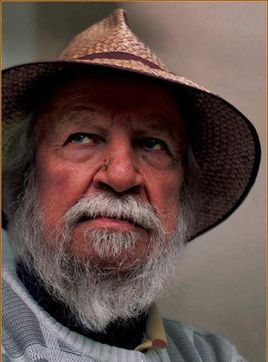
\includegraphics[scale=0.50]{images/2-2.jpg}
		\caption{威廉·戈尔丁}
		\label{fig2-2}
	\end{center}
\end{figure}
\begin{figure}[htb]
	\begin{center}
		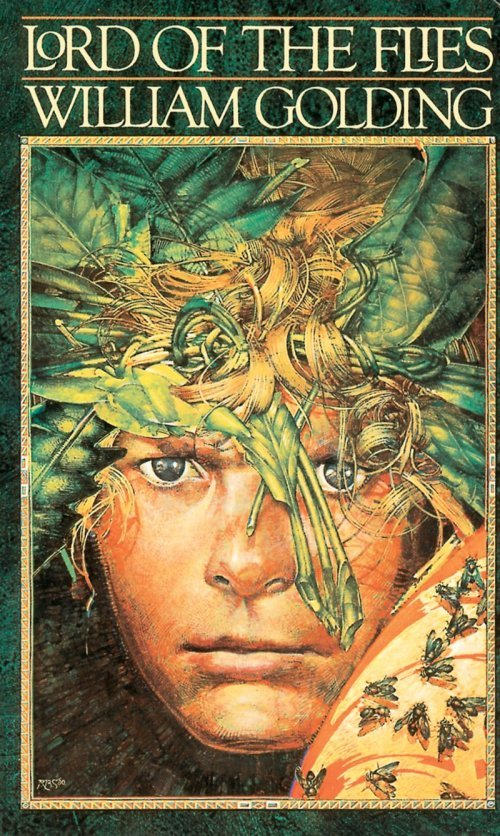
\includegraphics[scale=0.30]{images/2-4.jpg}
		\caption{蝇王}
		\label{fig2-4}
	\end{center}
\end{figure}
\subsection{内容简述}
故事的背景发生在一场未来的核战争下，一架飞机坠毁在一座荒岛上，机上的男孩们侥幸存活。
\\最初，孩子们在拉尔夫的领导下，以海螺作为权力象征，试图建立秩序，他们的主要目标是生存和发出求救信号等待救援。但好景不长，有序很快转为无序。搭建住棚和看守火堆这些工作很快让孩子们觉得被限制了个人自由，最后部分被刺激快感所吸引的孩子选择跟随杰克去打猎玩乐。
\\	至此，孩子们分为两帮，分别以拉尔夫和杰克为首。为了争夺对小社会的统治支配权，建立可以发号施令的权威，两派开始明争暗斗。在随之而来的斗争较量中，拉尔夫和猪崽一方被杰克和罗杰一方打得大败。失去了文明世界的理性和秩序，没有了纲纪规则，没有了互助合作，这群孩子完全堕落成一群嗜血的“野兽”。权力争斗的愈演愈烈及欲望和责任的冲突很快使孩子们文明有序的社会走向分裂。
\\	故事的结尾处，当杰克团体认定拉尔夫是仅剩的惟一叛逆者时，罗杰狰狞地削尖了木棒的两端，准备用对付野猪一样的手段来除掉拉尔夫。可怜的拉尔夫被追捕得四处乱窜，无处藏身，直到英国皇家海军舰艇经过荒岛相救，才幸免于难。故事的结局处，荒岛呈现出这样一幅悲伤凄惨的景象：“海岛已经全部烧毁，像块烂木头”，“拉尔夫的眼泪不禁如雨水般流了下来，他为童心的泯灭和人性的黑暗而悲泣。”

\subsection{内容启发}
一开始我不明白「蝇王」和作品有何联系，但后面我通过查阅资料，了解到其实“蝇王” 一词源于希伯来语 “Baalzebub”，在《圣经》中 “Baal” 被当作 “万恶之首”。至此，作品的深度才渐渐出显。
\\从作品中，我认为当中表出了人性的「丑恶」，或许无法用「丑恶」以形容，这仅仅是「天性」，而从用「孩童」的身份去定位当中的角色更能突显此「观点」，因为主观上往往不经世俗「洗礼」的孩童亦更接近于一个「纯真」的人，使其使接近「本能」地行动。所以，作品之中其实表现了人那与生俱来的「本能」。
\\紧接着的是告诉我们「规则」、「法律」的本质，为何故事的开始的秩序可以有条执行但不久却迎来崩解，是甚么导致了「秩序」的消落。在我看来，「秩序」本就不应存在，其本质只是人为所创造的工具，秩序的存在本来就是不公平的。「规则」的建立是取决于大部分人的标准，是为了维持利益的工具，而当这种规则与他人的行为相冲突时，秩序将迎来冲击。在作品中则以「本能」作表现，用「本能」这种极端的例子来说明「规则」对「人性」的压抑，而当「秩序」没有绝对的「力量」时，如作品般仅靠「道德」、「善良」应运而生的秩序显得是多么的无力不堪一击。
\\以上就是我对这部作品所理解的核心思想，点出了人的「本性」以及「规则」的本质及其影响。下面就基本完全是我自己对这两个主题的个人思想。希望带来启发，毕竟到一定年纪后才发现原来同龄人之间的三观亦能大相径庭。
因此想分享下自己的三观供以探讨批评。
\subsubsection{有感而發}
在我看来，秩序、法律、规则全都是因人而生的。如前面所说它们都是为了保障大部分人的利益而生的，因此，「秩序」的维持是需要力量的。然而，这并不能说明所谓的「正确性」和「合理性」。固然，「对」、「错」是主观的，当然亦可以认为「对」，「错」是存在的，毕竟这也是三观的一种。综上，我认为法律是「自私」的，因为它从来都只是以自己的标准去判断别人的对错，对别人进行所谓客观上的裁决。当然，这很符合现实生活。由始至终老师们常说的「换位思考」我认为并没有甚么作用，因为你只不过是把对方的行为演习多一次，整个过程都不过是在自己的世界观上进行，因为要你去理解对方的三观本身就是与自己作对的过程，何况这又费时同时对结果又没甚么影響。
\\说了那么多感觉其实并没有甚么意义，因为我深知我这一生是没有这「力量」去促使我对此方面进行改变，这样我和「小镇作题家」又何异﹖无可否认的是秩序为我带来了利益，我在议论的同时亦享受了它所带来的好处。世界上很多的事物亦是如此，是依附于「力量」的。固在欲想改变之前你最好拥有一定的力量去捍卫和建立你心中那不具有绝对正确性的公平。否则不过沦为笑谈以及迎来「正义」的审判。
\\我想强调的是有时候主流的思想不一定是正确的，希望自己可以记住这个道理拥有属于自己的看法或心得。对事物不要盲从，亦希望自己将来能够棱角依然。
\\下面将再介绍一些作品中小章节，篇幅不长但对我深有启发
	
	\section{《1984》——乔治·奥威尔}
	作者：乔治·奥威尔(\ref{fig2-3}見下圖)
	\\作品：1984(\ref{fig2-5}見下圖)
	\begin{figure}[htb]
		\begin{center}
			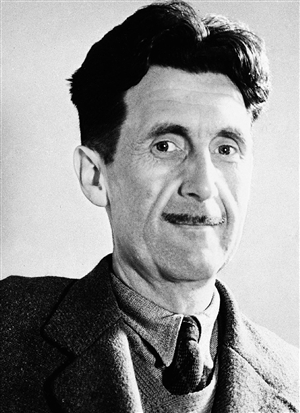
\includegraphics[scale=0.50]{images/2-3.jpg}
			\caption{乔治·奥威尔}
			\label{fig2-3}
		\end{center}
	\end{figure}
	\begin{figure}[htb]
		\begin{center}
			
\includegraphics[scale=0.30]{images/2-5.jpg}
			\caption{1984}
			\label{fig2-5}
		\end{center}
	\end{figure}
	
	\subsection{内容简述}
	“战争即和平，自由即奴役，无知即力量”——乔治·奥威尔
	\\在奥威尔虚构的极权主义国家 “大洋国” 中，温斯顿・史密斯是真理部的一名成员，他的工作是按照指示篡改历史资料。他开始对这个社会产生怀疑，并与茱莉亚私通，然而他们的幽会被思想警察发现，温斯顿被捕后遭受了残酷的折磨，最终被改造得服服帖帖，失去了自主思考的能力，成为了 “大哥” 的忠实信徒
	
	
	\subsection{内容启发}
	《1984》描绘的极权社会中，权力高度集中，思想被严格控制，人们的自由和尊严被剥夺。温斯顿的反抗和最终的屈服，深刻地展现了在极端环境下人性的脆弱和易被扭曲。在强大的政治压迫和思想洗脑面前，个人的意志和人性的美好被逐渐磨灭，揭示了极权主义对人性的扼杀，以及人们在这种环境下为了生存而不得不放弃自我、屈从权威的悲哀，引发了人们对自由、权力与人性关系的深入探讨。
	\\「历史」能够被篡改吗，篡改后的历史还能算是「历史」吗，这个问题从作品带入到现实，就目前事实而言，的确出现了不同教材对同一事件的不同描述。何者才是真理，这个问题将永恒存在，谁也无法断言。因此，我认知历史的方式只是暂时相信我所认为的主流学说，不能排除历史被推翻的一天，虽然说要相信科学，但我时常幻想，恐龙是否真实存在过，我们所见到的证据是否不过是前人的雕塑作品。因此，我认为我们应该对历史始终保持待定的态度。

	\section{《巴别塔》——圣经}
	來源：圣经(\ref{fig2-6}見下圖)
	\begin{figure}[htb]
		\begin{center}
			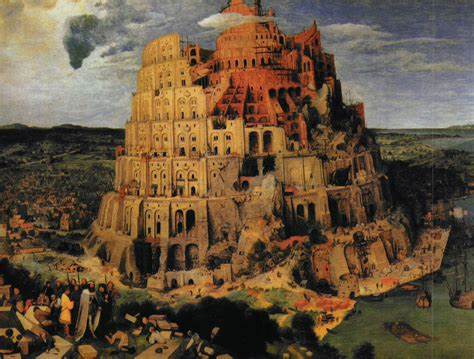
\includegraphics[scale=0.60]{images/2-6.jpg}
			\caption{巴別塔}
			\label{fig2-6}
		\end{center}
	\end{figure}
	
	\subsection{内容简述}
	在《圣经》中，大洪水过后，人类说着同一种语言，他们向东迁移，在示拿地（Shinar）发现一片平原，于是决定在那里建造一座城和一座通天塔，来传扬人类自己的名声，免得人类分散在全地上。
	\\上帝降临，看到人类所建造的城和塔。他说：“看哪，他们成为一样的人民，都是一样的言语，如今既做起这事来，以后他们所要做的事就没有不成就的了。” 于是，上帝决定变乱人类的语言，使他们彼此言语不通。人们因为无法沟通交流，建造工作被迫停止，人类也就分散在世界各地。
	
	\subsection{内容启发}
	这并非算得上我所喜欢的故事，但其内涵的确震撼到我了，这个故事有很多不同的解释，下面选一个我喜欢的版本来解读启发。
	\\首先，「巴别塔」名字的由来就带有“变乱”的意思，是人类向上帝，向权威挑战的精神结晶，同时「巴别塔」亦是人类的幸褔之塔。在建塔的过程中融入了人们的希望，象征了人类对幸褔美好的向往。
	\\但同时亦突显出了人类的骄傲和过度的野心受到了惩罚。从这个角度看，妄图和神平起平坐本身就是不现实的，巴别塔更多地象征着人类的狂妄自大和不切实际的幻想。它提醒人们要认识到自己的局限性，过度的自负往往会带来失败和灾难。
	
\section{总结感悟}

坦白来说我并不热衷于解读作品的含意，很多时候只是当消遣娱乐，的而且确有时深思可以带来启发，但的确自己对无法共呜的作品难以起兴，或许这就是我之所以为平凡人的原因。我认为其原因是因为我目前的三观经已建立起基础，对一定的见解基本己落实自己的是非观。因此在主流的三观问题上我不会探讨太多。我意思是可以有不同的三观，我亦承认你的思想，只是这三观或许无法使我改变。
\\所以看的作品往往看到的只是自己想看的角度。但这并非意思我的三观不会再有所改变，当遇到一些「好」的思想时我亦会学习，何谓「好」我难以描述，但基本上思想的改变往往来自于我从冲击中发现了自己三观的缺失。但在这个过程中往往是不理性的，所以我只能尽可能地提醒自己要客观地看待事物。
\\我感觉目前自己的三观并没有太大动摇，但我的意志的确开始变动了，我不喜欢「虚无主义」这个词，所以我亦不想承认我的三观是与「虚无主义」有所关系，但的确在我的三观中经早已接受并理解了“思想没有对错”这一观念，我想这个观念已经无法再改变了。因此显得自己对三观上的态度十分随意。年时的我觉得精神世界对我十分重要，直到现在我亦十分认可，但随着年纪越来越大，我开始有了更多的地方要考虑，有点无力维持心之所向，同时亦是自己迷茫的一种表现。只希望自己能仍记初心，锐气不减。

\end{document}